\documentclass[Main]{subfiles}
\begin{document}


\section{System components}

In Figure \ref{fig:ComponentsAndInterfaces} an overview of the complete system's components and interfaces is shown.
Each component and interface will described and linked with system requirements in the following subsections.

\begin{figure}[H]
\centering
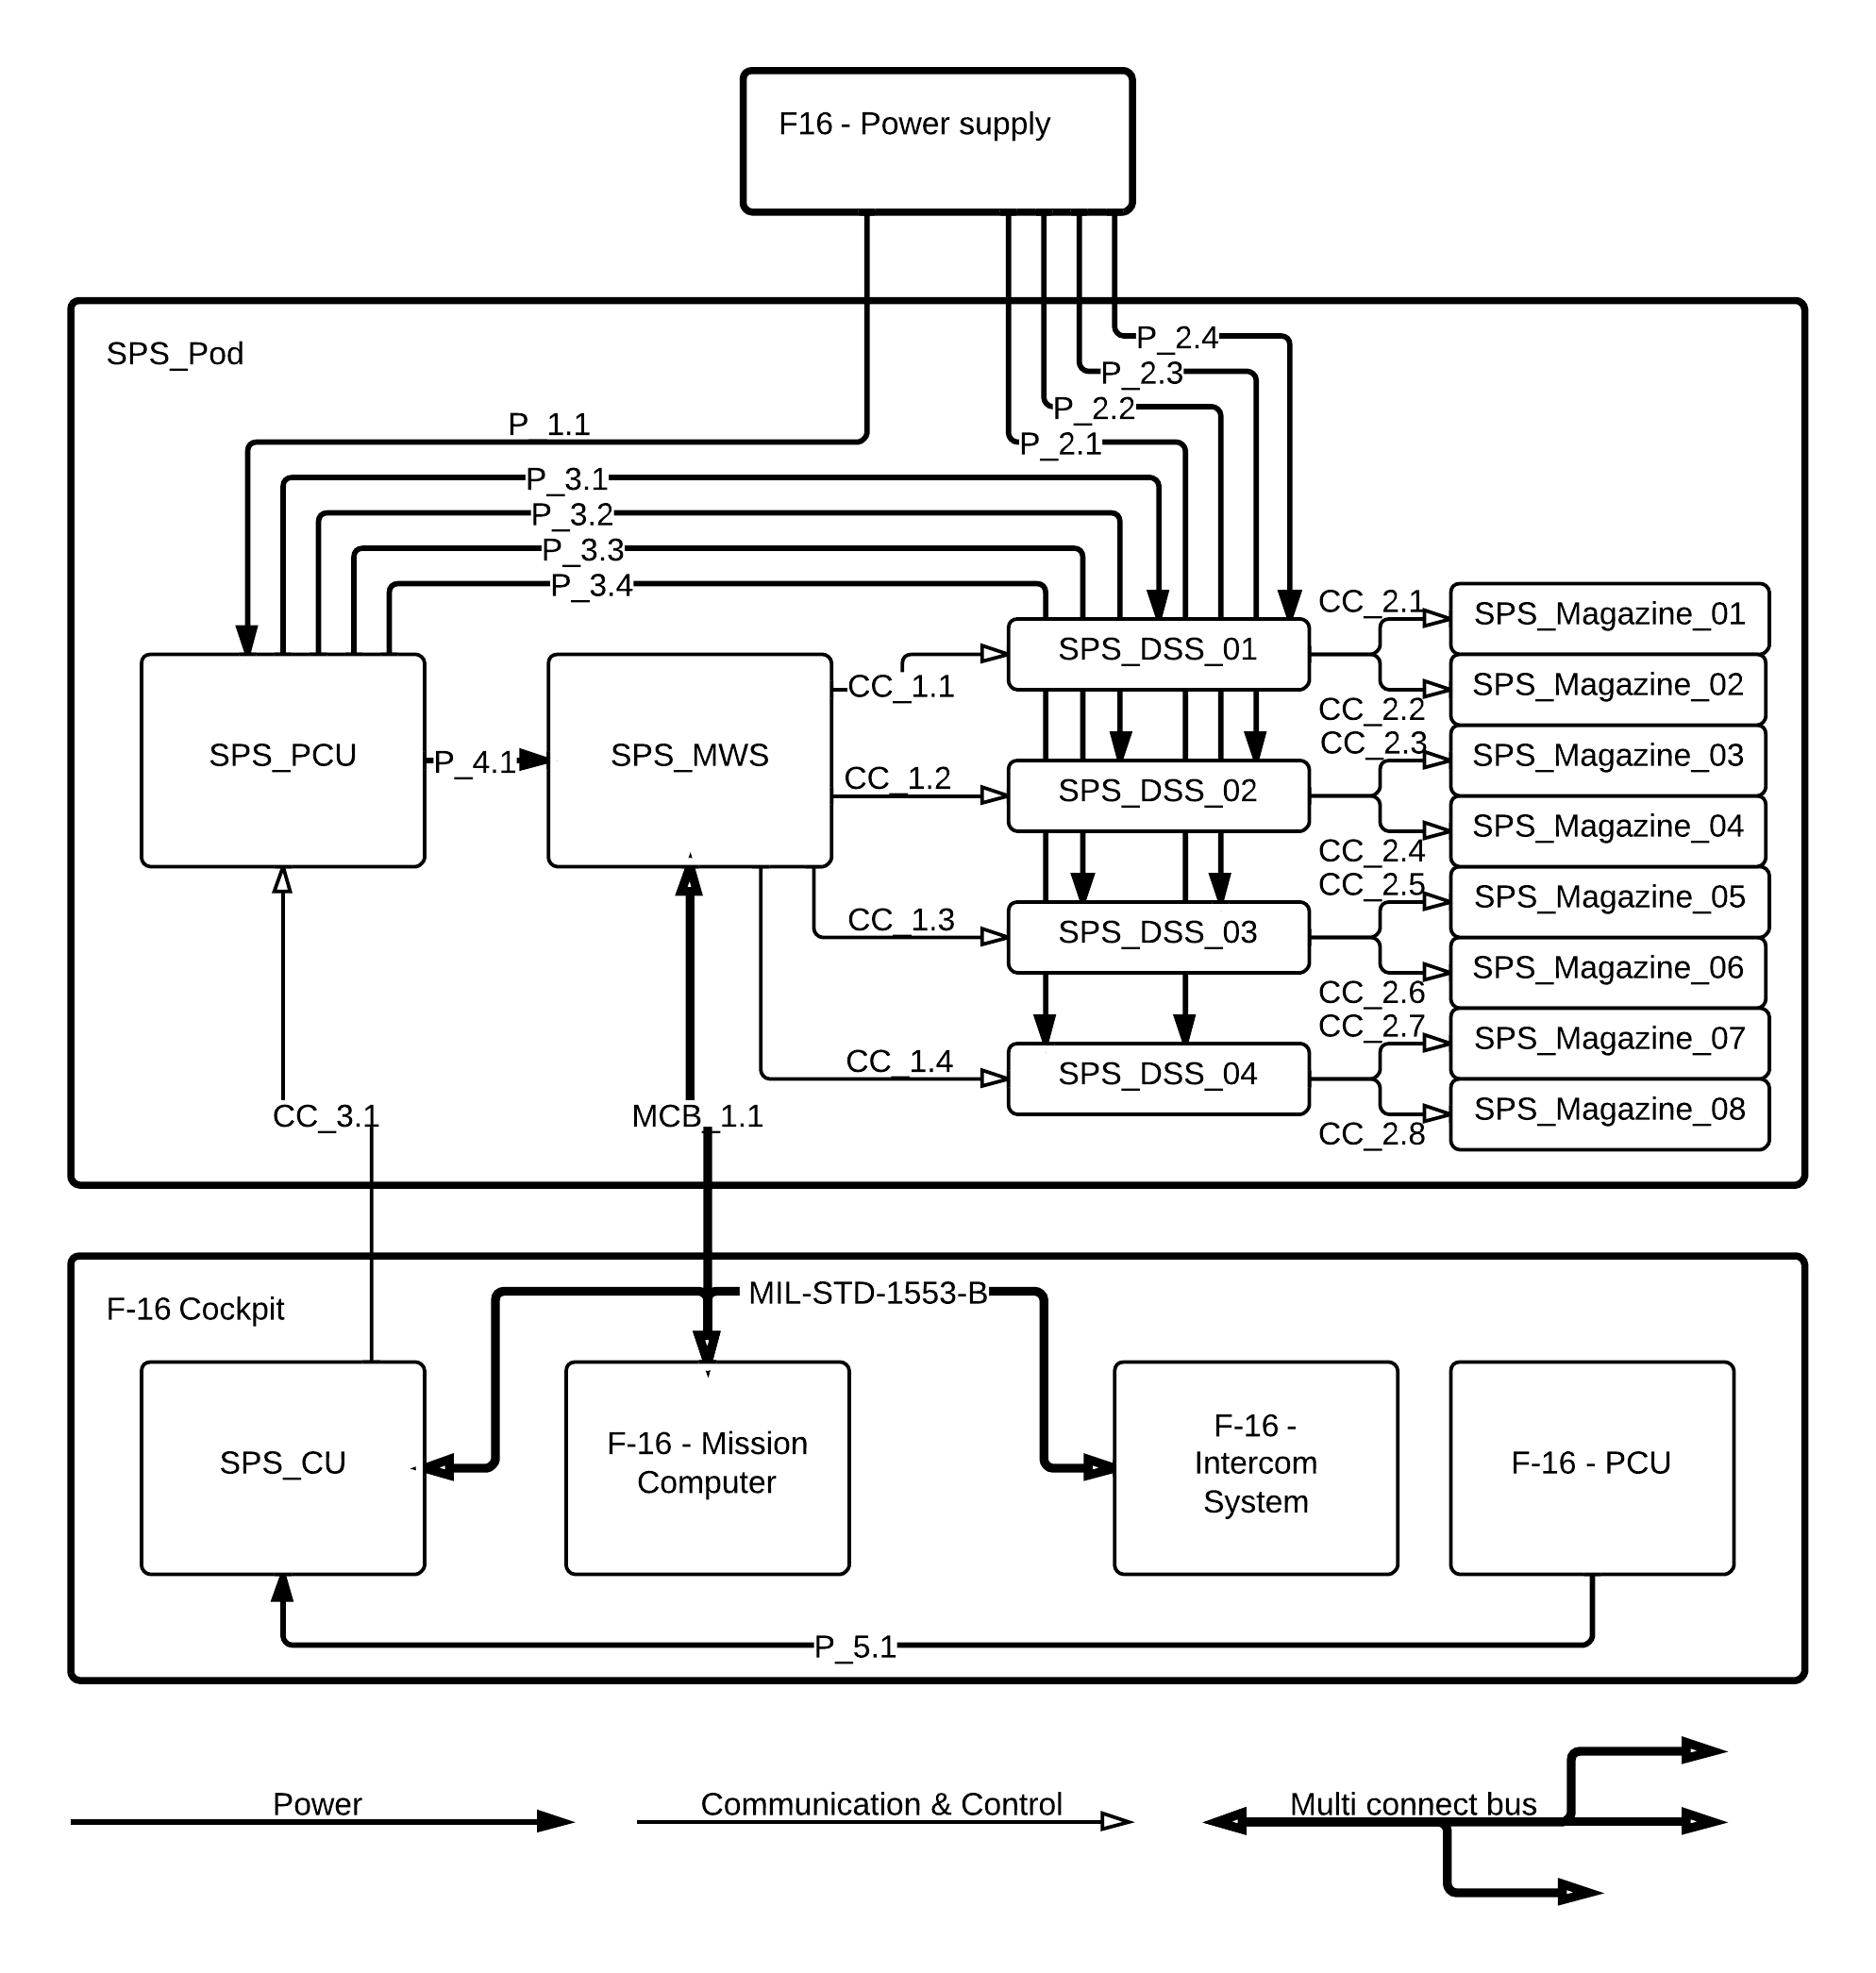
\includegraphics[width = 0.9\textwidth]{ComponentsAndInterfaces}
\caption{Components and interfaces}
\label{fig:ComponentsAndInterfaces}
\end{figure}

\subsection{F-16 Power Supply}
The F-16 Power Supply is capable of delivering 700W with a voltage of 115 VAC 400 Hz. It distributes power to the other components (F.5).

\subsection{F-16 Mission Computer}
The F-16 Mission Computer is responsible for telling the Cockpit Unit when the aircraft is on the ground so it can lock dispensing of payloads (F.13).

\subsection{SPS\_POD}
The pod structure support the weight of all its internal components (F.6).

\subsection{SPS\_PCU}
The Power Conditioning Unit is responsible for receiving high voltage AC power from the F-16 power supply, converting it to low voltage DC power and distributing it to the MWS and the DSS's (F.8).

\subsection{SPS\_MWS}
The Missile Warning System is responsible for monitoring the planes surroundings for incoming missiles (F.7).
When a missile is identified as being in the path of the plane, the MWS will signal the F-16 mission computer in order to let the pilot take appropriate action (F.10).
Additionally it will signal the F-16 intercom system (F.11).

\subsection{SPS\_DSS\_XX}
The Digital Sequencer Switches are responsible for powering and firing chaff/flare magazines on command from the MWS (F.9).

\subsection{SPS\_Magazine\_XX}
The magazines contains the payloads to be dispensed (F.4).

\subsection{SPS\_CU}
The Cockpit Unit receives input from the pilot (F.1, F.2, F.12) and communicates with the MWS and the mission computer.

Loading of preprogrammed patterns is done through the Cockpit Unit (F.3).

Through input from the User, the Cockpit Unit can turn on/off power to the pod (F.14).

The Cockpit Unit is responsible for controlling and validating dispensing of payloads (F.15).


\end{document}
